%! TeX program = lualatex
\documentclass[../main.tex]{subfiles}
\begin{document} \section{The limit laws}
We learned how to estimate limits of functions. We now learn how to \hlsupp{evaluate} limits \emph{exactly}.

  % \faExclamationTriangle{} This section covers a bit more than the corresponding textbook section and is organized differently to minimize redundancy. See the last page for a short comparison.

\begin{mdframed}[style=simple-compact]
  If \(f(x)\) is a polynomial or a rational function, then
  \[
    \lim_{x \to a} f(x) = f(a).
  \]
\end{mdframed}
\faExclamationTriangle{} Note \(a\) must be a constant \underline{\hspace{6cm}} and \underline{\hspace{2in}}.
% Note that a must be in the domain of f and is not an infinity.
% DO NOT DO arithmetic with infinity.  

\blanklines{5}

\begin{example}
  Evaluate \(\lim_{x \to -2} x^{2} + 5 x^{3}\).

  \blanklines{5}
\end{example}

% \faExclamationTriangle{} If your intuition from high school leads to doing arithmetic with infinities, then that's a good sign that you need to use limit laws explicitly.

We need to use limit laws whenever direct substitution does not apply.
\begin{mdframed}[style=withref-compact]
  \textbf{Theorem} (Limit Laws). Suppose \(\lim_{x \to a} f(x)\) and \(\lim_{x \to a} g(x)\) \hlwarn{both exist}. Then
  \begin{enumerate}[label=(\arabic*)]
    \item \(\lim_{x \to a} [f(x) + g(x)] = \lim_{x \to a} f(x) + \lim_{x \to a} g(x)\) \hfill (sum)
    \item \(\lim_{x \to a} [f(x) - g(x)] = \lim_{x \to a} f(x) - \lim_{x \to a} g(x)\) \hfill (difference)
    \item \(\lim_{x \to a} [c \; f(x)] = c \lim_{x \to a} f(x)\), where \(c\) is a constant \hfill (constant multiple)
    \item \(\lim_{x \to a} [f(x) \; g(x)] = \lim_{x \to a} f(x) \cdot \lim_{x \to a} g(x)\) \hfill (product)
    \item \(\lim_{x \to a} \frac{f(x)}{{\color{warn} g(x)}} = \frac{\lim\limits_{x \to a} f(x)}{{\color{warn} \lim\limits_{x \to a} g(x)}}\), \quad \hlwarn{if {\(\lim_{x \to a}g(x) \ne 0\)}} \hfill (quotient)
    \item \(\lim_{x \to a} \bigg[f(x)\bigg]^{n} = \bigg[ \lim_{x \to a} f(x) \bigg]^{n}\) \hfill (power)
    \item \(\lim_{x \to a} \sqrt[n]{f(x)} = \sqrt[n]{\lim_{x \to a} f(x)}\), \quad if \(n\) is even, we assume {\(\lim_{x \to a} f(x) \ge 0\)} \hfill (root)
  \end{enumerate}

  \textbook{Theorem 2.5 Limit Laws on page 161}
\end{mdframed}

\faStar{} All limit laws apply to \hlmain{one-sided} (of the same type) as well as \hlmain{two-sided} limits.

\blanklines{5}

% Tips: 
% \begin{enumerate*}[label=(\alph*)]
%   \item Group the constant multiple and the product laws together because a constant multiple is also a product.
%   \item A power is just a repeated product. Therefore, the power law is a special case of the product law.
%   \item Group the root and the power law together because \(\sqrt[n]{\cdots} = (\cdots)^{1/n}\).  They come from the same theorem anyway.
% \end{enumerate*}

\clearpage

Applying limit laws correctly is all about decomposing a function along algebraic operations to break up a larger task into smaller tasks. At the very end, we only evaluate limits of very simple functions such as polynomial and rational functions. The rest will be arithmetic.
\begin{example}
  Let \(f(x) = \sqrt[5]{x^{2} + 1} - 2 (4x - 3)^{100}\). Evaluate \(\lim_{x \to 1} f(x)\).

  \blanklines{40}
\end{example}

\faExclamationTriangle{} As far as grading is concerned, we are expected to \hlwarn{show details of calculations} in assignments, tests and the final exam.  Unless stated otherwise, solutions (to short and long answer questions) without details or sufficient justification will typically be given \(0\), regardless of correctness. 
\clearpage

Limit laws are still useful when only abstract information is available.
\begin{example}
  Suppose \(\lim_{x \to -3} f(x) = 4\). Evaluate \(\lim_{x \to -3} \left( f(x) \right)^{3/2}\) if possible.

  \blanklines{10}
\end{example}

A variation-on-the-theme problem.  
\begin{exercise}
  Let \(c\) be an unknown constant. Suppose \(\lim_{x \to 1} \sqrt{2x^{3} + cx - 1} = 3\). Find \(c\).

  \blanklines{10}
\end{exercise}

Remember that limit laws also apply to one-sided limits (of the same type) and piecewise functions.
\begin{example}
  Let \(f(x) = \begin{cases}\sqrt{x - 1} + 1, &x > 1\\[1ex]\frac{2x}{x + 1}, &x < 1\end{cases}\). Evaluate \(\lim_{x \to 1} f(x)\).

  \blanklines{18}
\end{example}

\clearpage
We now get into the more demanding territory of \hlmain{combining limit laws and algebra skills} to evaluate limits where the limit laws seemingly don't apply \hlsupp{at first glance}.

\begin{example} \label{ex:limit-cancellation}
  Evaluate \(\lim_{t \to 2} \frac{t^{2} - 3t + 2}{t - 2}\) or explain why it does not exist.

  \blanklines{20}
\end{example}

\begin{example} \label{ex:limit-rationalization}
  Evaluate \(\lim_{x \to 0} \frac{\sqrt{x^{2}+1}-1}{x^{2}}\) or explain why it does not exist.

  \blanklines{25}
\end{example}
\clearpage

Example~\ref{ex:limit-textbook-2.28} is a subtle variation on the theme of Examples~\ref{ex:limit-cancellation} and \ref{ex:limit-rationalization} but challenges our algebra skills even more. It is a really good practice, but leave it until you have mastered all other skills. Hopefully, the hint at the bottom of the page helps.
\begin{exercise}[Textbook Example~2.20] \label{ex:limit-textbook-2.28}
  Evaluate \(\lim_{x \to 0} \frac{1}{x} + \frac{5}{x(x-5)}\) or explain why it does not exist.

  \blanklines{20}
\end{exercise}

Example~\ref{ex:limit-infinity-plus-constant} looks similar to Examples~\ref{ex:limit-cancellation} and \ref{ex:limit-rationalization} but is much simpler.
\begin{exercise} \label{ex:limit-infinity-plus-constant}
  Evaluate \(\lim_{x \to 0^{-}} \frac{x+1}{x(x-1)}\) if it exists.

  \blanklines{18}
\end{exercise}

\vfill{}
{\scriptsize Hint to Example~\ref{ex:limit-textbook-2.28}}. \newline
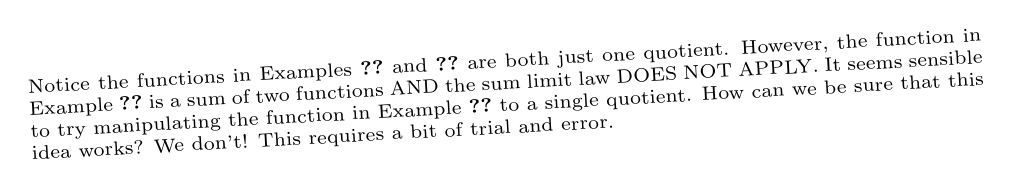
\begin{tikzpicture}[scale=1]
  \node[rotate={pi}, inner sep=0pt] {\parbox{\linewidth}{\scriptsize Notice the functions in Examples~\ref{ex:limit-cancellation} and \ref{ex:limit-rationalization} are both just one quotient. However, the function in Example~\ref{ex:limit-textbook-2.28} is a sum of two functions AND the sum limit law DOES NOT APPLY. It seems sensible to try manipulating the function in Example~\ref{ex:limit-textbook-2.28} to a single quotient. How can we be sure that this idea works? We don't! This requires a bit of trial and error.}};
\end{tikzpicture}
\clearpage

Exercise~\ref{ex:limits-strategy} encourages you to make connections (compare, contrast, summarize, synthesize ideas) among techniques we have learned so far.
\begin{exercise} \label{ex:limits-strategy}
  Find \hlmain{a strategy} that works for all these limits.  By strategies, we mean the way techniques can be combined and patterns in the form of functions (\emph{not} patterns in numbers). Work in groups. Experiment with different methods. Trial-and-error is a good learning activity.
  \[
    L_{1} = \lim_{x \to 1} \frac{x^{2}-1}{x-1}, \qquad
    L_{2} = \lim_{x \to 4} \frac{\sqrt{x}-2}{x-4}, \qquad
    L_{3} = \lim_{x \to 1} \frac{x^{1/3}-1}{x-1}.
  \]
  Getting the final numerical answers is not the point. Note \(L_{1} = 2, L_{2} = 1/4\) and \(L_{3} = 1/3\).

  \blanklines{45}
\end{exercise}

\clearpage

\begin{mdframed}[style=withref]
  \textbf{The Squeeze Theorem}. Let {\(f(x) \le g(x) \le h(x)\)} when \(x\) is near \(a\) (except possibly at \(a\)) and
  \[ { \lim_{x \to a} f(x) = \lim_{x \to a} h(x) = L,} \]
  then
  {\(\lim_{x \to a} g(x) = L\).}

  \textbook{Theorem 2.7 on page 171}
\end{mdframed}

\begin{example} \label{ex:limit-law-x-square-sin(x)}
  Evaluate \(\lim_{x \to 0} x^{2} \sin\left(\frac{1}{x}\right)\).

  \blanklines{30}
\end{example}
\clearpage

Exercise~\ref{ex:limit-law-x-sin(x)} is only a tad different from Example~\ref{ex:limit-law-x-square-sin(x)} but requires a few more steps.
\begin{exercise} \label{ex:limit-law-x-sin(x)}
  Evaluate \(\lim_{x \to 0} x \sin\left(\frac{1}{x}\right)\).

  \hfill\includestandalone[width=2in]{../standalones/plot_squeeze}

  \begin{enumerate}[wide]
    \item We will apply the Squeeze Theorem.  The form of \(x \sin(1/x)\) suggests that we choose
      \begin{itemize}
        \item the lower bound to be \(f(x) = \underline{\hspace{1in}}\),
        \item the upper bound to be \(h(x) = \underline{\hspace{1in}}\).
      \end{itemize}

    \item Sketch your choices of \(f(x)\) and \(h(x)\) on the graph above. Do they \enquote{squeeze} \(x \sin(1/x)\)? If so, move on to the next step; otherwise, go back to the previous step and try again.

      Hint: \(f(x) = -x\) and \(h(x) = x\) are the wrong choices.

  \item The choices for \(f(x)\) and \(g(x)\) forces us to show \(f(x) \le x \sin(1/x) \le g(x)\) in two steps. 
    \begin{enumerate}
      \item Show that \(f(x) \le x \sin\left(\frac{1}{x}\right) \le h(x)\) \hlwarn{for \(x \ge 0\)}.

        \blanklines{10}

      \item Show that \(f(x) \le x \sin\left(\frac{1}{x}\right) \le h(x)\) \hlwarn{for \(x < 0\)}.

        \blanklines{10}
    \end{enumerate}

  \item Apply the Squeeze Theorem to finish evaluating the limit.

    \blanklines{4}
  \end{enumerate}
\end{exercise}
\clearpage

\begin{exercise}
  Suppose \(x+1 \le g(x) \le x^{3} - 2x + 3\). Find \(\lim_{x \to 1} g(x)\).

  \blanklines{45}
\end{exercise}

\end{document}

